\section{Vlastní řešení}

\subsection{Koncepce}
Chtěl bych vytvořit otevřenou IoT Platformu, která bude určeta pro nejrůznější kutily s elektronikou a technické nadšence. K dispozici bude zdarma veřejná instance sloužící primárně pro uživatele, kteří si chtějí Platformu jednoduše a rychle vyzkoušet a nebo chtějí provozovat pouze pár zařízení. Pro ty kteří chtějí mít plnou kontrolu nad svými daty a být nezávislý na připojení k internetu, bude k dispozici možnost hostingu celého řešení na vlastním hardwaru. K Platformě půjde připojit různorodá zařízení a bude vytvořeno schéma pomocí kterého zařízení popíší Platformě vlastní funkčnost/schopnosti. Na základě těchto informací se automaticky uživateli vygeneruje webové rozhraní ke sledování a ovládání jeho zařízení.

Na bezpečnost bude kladený vysoký důraz. Primárně bude založená na uživatelských účtech, které budou mít oprávnění pouze ke svým zařízením, případně těm ke kterým dostali oprávnění od jiných uživatelů. Každý uživatel by měl mít k dispozici vlastní prostředí, v rámci kterého budou jeho zařízení komunikovat. Uživatel si bude moci snadno přihlásit k odběru této komunikace a tak sledovat všechny zprávy posílané mezí zařízeními a Platformou.


\subsection{Popis domény} % nativní podpora pro switch, sensor, generic - jednolivé popsat, abych se mohl na ně odkázat v UC
Tato kapitola obsahuje popis jednotlivých entit/pojmů se kterými Platforma pracuje.
\begin{figure}[htbp]
    \label{domain-model}
    \centering
    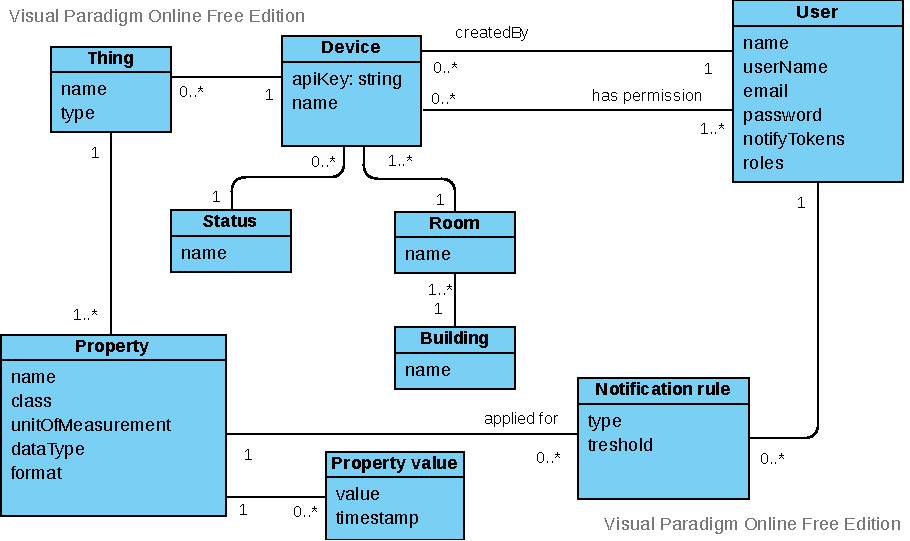
\includegraphics[width=\textwidth]{img/domain.pdf}
    \caption{Doménový model}
\end{figure}
\begin{itemize}
    \item \textbf{Uživatel (User)} - fyzická osoba, která interaguje se systémem přímo pomocí pomocí uživatelského rozhraní.
    \item \textbf{Zařízení (Device)} - fyzické zařízení, které komunikuje s Platformou, dále se dělí na Věci
    \item \textbf{Věc (Thing)} - logické uskupení Vlastností, např. meteostanice
    \item \textbf{Vlastnost (Property)} - určitá veličina, jejíž hodnota se odesílá na Platformu (např. teplota), která případně umožňuje být Platformou změněna/nastavena
    \item \textbf{Umístění (Location)} - kde je dané zařízení umístěno, specifikující budovu a místnost, např. doma-kuchyňe
    \item \textbf{Stav Věci (State)} - v jakém aktuálním stavu se určitá Věc nachází, skládá se ze stavů příslušných Vlastností
    \item \textbf{Notifikační pravidlo (Rule)} - za jaké podmínky se má uživateli odeslat notifikace
\end{itemize}


\subsection{Případy užití}
Tato kapitola popisuje identifikované případy užití, které současně slouží jako podklad funkčních požadavků kladených na řešení. Figurují v nich následující aktéři:
\begin{itemize}
    \item Uživatel - představuje autentizovaného uživatele webového rozhraní.
    \item Administrátor - představuje autentizovaného uživatele s nejvyšším stupněm oprávnění.
    \item Zařízení - představuje koncové zařízení komunikující s Platformou
\end{itemize}

\begin{figure}[htbp]
    \centering
    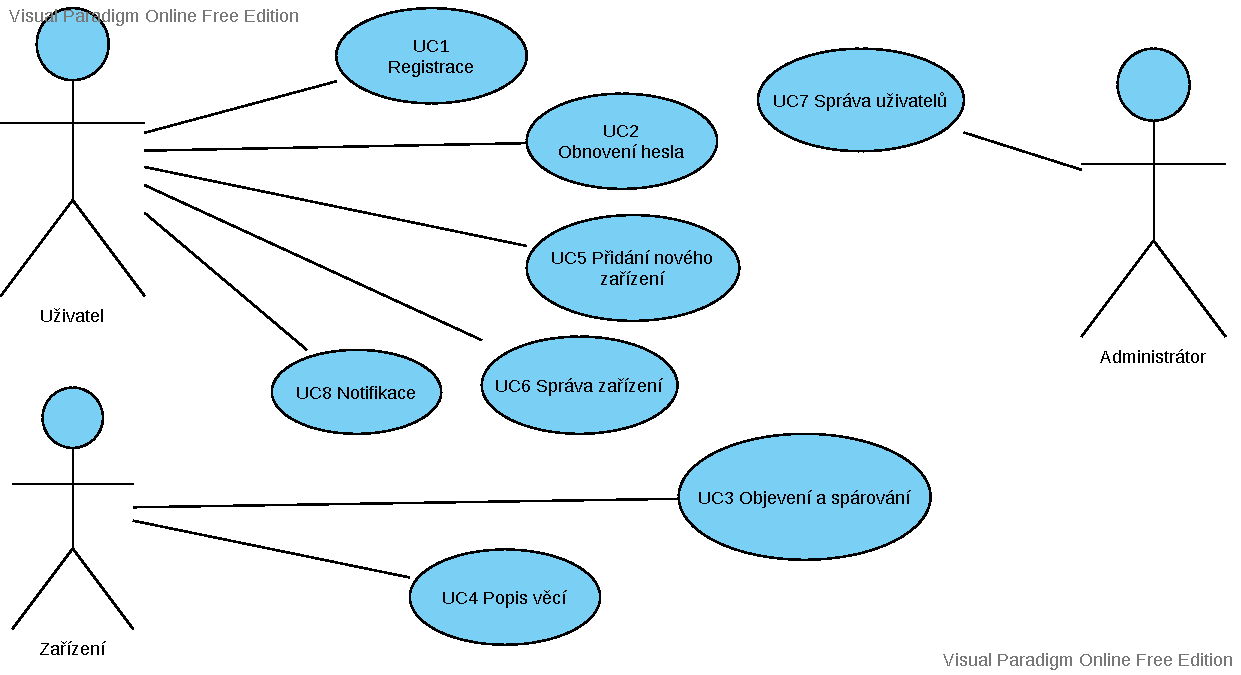
\includegraphics[width=0.7\textwidth]{img/use_case.pdf}
    \caption{Případy užití}
\end{figure}

\paragraph{UC1 Registrace uživatele}
- neautentizovaný uživatel vyplní registrační formulář obsahující jméno, přijmení, uživatelské jméno, heslo a email. Při zpracování požadavku na serveru bude zajištěna unikátnost uživatelského jména a emailu napříč databází. Uživatel bude informován o úspěchu/neúspěchu akce. Po úspěšné registraci bude automaticky přihlášen, pokud nezrušil ve formuláři zaškrtávátku \uv{Automaticky přihlásit}, a bude mu odeslán uvítací email na zadanoou emailovou adresu.

\paragraph{UC2 Obnovení hesla}
- součástí přihlašovacího formuláře bude odkaz na stránku pro obnovení zapomenutého hesla, kde bude uživatel dotázán na emailovou adresu, kterou použil při registraci. Po zadání, pokud daná emailová adresa je součástí některého uživatelské účtu, bude na ni odeslán email s odkazem pro obnovu hesla. Na tomto odkazu bude uživatel vyzván k zadání nového hesla.

\paragraph{UC3 Objevení a spárování nového zařízení}
- zařízení, pokud není ještě není spárované s Platformou, tak po zapnutí vyzve uživatele k zadání svéhu uživatelského jména na Platformě. Toto zadání bude umožněno vytvořením Wifi přístupového bodu, na kterém poběží kaptivní portál - po připojení telefonem/počitačem se automaticky zobrazí webová stránka s formulářem pro zadání údajů. Následně se zařízení připojí k Platformě, ohlásí jaké má Věci, popíše jejich Vlastnosti, a bude ji informovat, kterému uživateli (podle zadaného uživ. jména) má zobrazit možnost přidání nového zařízení. Pokud si uživatel dané zařízení přidá (viz. \hyperref[UC5]{UC5}), tak následně Platforma odešle zařízení API klíč, které si ho uloží a přihlásí se pomocí toho klíče k Platformě (nyní je spárované).

\paragraph{UC4 Popis věcí}
- zařízení při ohlašování definice věcí a jejich vlastností musí oznámit mimo jiné typ věci. Platforma bude podporovat kromně generického (generic) typu další 3 typy věcí, pro které bude speciální zobrazení v uživatelském rozhraním:
\begin{itemize}
    \item Switch - přepínač, který se nachází ve stavu on/off. V rozhraní bude Věc reprezentována dvou stavovým přepínačem, který při kliknutí odešle změnu o stavu na druhý než ve kterém se aktuálně nachází. (využití např. vypínač světla)
    \item Activator - spínač, který má pouze jeden stav. V rozhraní bude věc reprezentována tlačítkem, které na stisk odešlě aktivaci zařízení. (využití např. ovladač pojízdné brány)
    \item Sensor - v rozhraní bude reprezentován jako widget zobrazující aktuální hodnota první vlastnosti. Po rozkliknutí se zobrazí graf vizualizující průběh hodnoty v čase za posledních 24h.
    \item Generic - obecný typ u kterého zařízení popíše strukturu, datové typy a názvy příslušných vlastností. V uživatelském rozhraní bude věc reprezentována jako Widget, který po kliknutí zobrazí Dialogové okno umožňující zobrazení a ovládání všech vlastností dle konfigurace.
\end{itemize}


\paragraph{UC5 Správa zařízení}
\label{UC5}
- uživatel na stránce \uv{Správa zařízení} bude mít tyto dvě sekce:
\begin{itemize}
    \item \uv{Přidat zařízení} - zde se zobrazí všechna nově detekovaná zařízení, která ještě nemá přidaná. Následně při kliknutí na tlačítko přidat se zobrazí jednoduchý formulář pro zadání umístění a názvu zařízení - bude předvyplněn název, který ohlásilo zařízení. Uživatel formulář potvrdí, systém následně vytvoří dané zařízení, přidá uživateli k němu oprávnění a ná stránce \uv{Ovládání} už bude uživatel moci sledovat aktuální stav Věcí a případně je i ovládat (pokud to umožňují).
    \item  \uv{Správa} - zde budou zobrazena všechna zařízení, ke kterým má uživatel oprávnění. Rozhraní umožní pro každé zařízení, ke kterému má právo pro editaci, jeho smazání a pomocí formuláře editaci - názvu, umístění a změnu oprávnění pro jednotlivé uživatele. Tyto oprávnění budou rozděleny na tyto tři úrovně:
          \begin{itemize}
              \item \textbf{Read} - uživatel může si zobrazit veškeré údaje o zařízení.
              \item \textbf{Control} - uživatel může zařízení ovládat.
              \item \textbf{Write} - uživatel může editovat veškeré informace o zařízení (včetně oprávnění).
          \end{itemize}
\end{itemize}

\paragraph{UC6 Správa uživatelů}
- administrátor může přistoupit na stránku \uv{Správa uživatelů}, kde se mu zobrazí seznam všech registrovaných uživatelů. Jednotlivé uživatele může smazat a pomocí formuláře editovat všechny jejich osobní údaje včetně hesla.

\paragraph{UC7 Notifikace}
- rozhraní umožní uživateli nastavit pravidlo pro libovolnou věc, při kterém se odešlě Web Push notifikace na jeho zařízení. Pro nastavení bude zobrazený formulář umožňující výběr z vlastností dané věci, po vybrání se zobrazí výběr akce, při jejímž splnění chce uživatel obdržet notifikaci (překročení hodnoty / vždy / hodnota bude rovna) a případné pole pro zadání limitní hodnoty. Dále půjde zobrazit rozšířené nastavení pro konkrétní notifikační pravidlo umožňující nastavení času a konkrétních dní v týdnu, kdy bude pravidlo platné (ve výchozím stavu bude vždy). Těchto pravidel si bude moci nastavit libovolný počet pro každé zařízení, ke kterému má oprávnění pro čtení.



\subsection{Nefunkční požadavky}

\paragraph{N1 Řešení spustinelné na Linux systému}
- systém bude možno provozovat na Linuxovém serveru (Debian) a také na platformě Raspberry Pi (verze 3B+/4, OS Raspbian).

\paragraph{N2 Responzivní webové rozhraní}
- aplikace bude nabízet responzivní webové uživatelské rozhraní přizpůsobené pro zobrazení na mobilních zařízeních i stolních počítačích. Uživatelské rozhraní bude kompatibilní s prohlížeči Mozilla Firefox verze 80, Chrome verze 80 a Safari na iOS. Dále bude implementovat tzv. PWA (Progresivní webová aplikace) - bude využívat cache pro statické soubory pro rychlé načítání, spustitelné offline a na zařízení Android půjde v aplikaci chrome přidat na plochu a následně vypadat jako nativní aplikace.

\paragraph{N3 Rozhraní realizováno jako SPA}
- SPA (Single page application) je webová aplikace, která utilizuje JavaScript, aby při interakci v rámci aplikace se nemusela celá stránka načítat, ale pouze chytře překresluje potřebné části. Výsledkem je mnohem přijemnější uživatelský zážitek, než při čekání na stažení a překreslení celé stránku po kliknutí na odkaz.

\paragraph{N4 Validace}
Uživatel při vyplňování veškerých formulářů v uživatelském rozhraní obdrží interaktivní zpětnou vazbu v případě zadání nevalidních údajů. Interaktivní vazbou jsou myšleny následující scénáře při průchodu formuláře:
\begin{itemize}
    \item Zadání nové hodnoty a vykliknutí z pole - bude provedena validace a v případě nevalidního vstupu, bude uživatel vizuálně  upozorněn.
    \item Editace již zadané hodnoty v poli - validace bude provedena po každé změně (stisknutí klávesy), uživatel bude opět vizuálně upozorněn v případě nevalidního vstupu.
\end{itemize}

\paragraph{N5 Koncová zařízení na platformě ESP8266}
- pro jednotlivá zařízení bude použit čip ESP8266 od firmy Espressif jako mikrokontroler, který bude komunikovat po sítí prostřednictvím Wifi sítě.

\paragraph{N6 Výkonnostní požadavky}
- systém bude stabilní a zvládne obsluhovat stovku zařízení, kde každé bude odesílat změnu stavu s periodicitou 30 vteřin. Při tomto dlouhodobém zatížení nebude docházet k pádům systému ani k výraznému zpoždění komunikace (RESTful požadavky pod 200 ms).

\paragraph{N7 Konfigurace systému}
- veškerá konfigurace (týkající se externích služeb/komunikace) jako jméno a heslo do databáze, číslo portu pro komunikaci atd. bude konfigurovatelné pomocí promněných prostředí (env variables). Detailní popis promněných bude obsažen v instalační příručce.


\subsection{Vybrané technologie}

\subsubsection{Komunikační protokol}   %https://ieeexplore.ieee.org/abstract/document/8079928
Komunikační protokolů je velké množství a přímo závisí na výběru přenosného média. Při použití specializovaných sítí jako LoRa nebo Zigbee, nemáme moc velkou flexibilitu ve výběru. Zařízení podporující tyto specializované sítě jsou poměrně drahá, ale umožňují běh na baterii. Zatímco využití WiFi sítě nám dává obrovskou flexibilitu ve výběru protokolů a zařízení podporující připojení k Wifi nebyli nikdo více cenově dostupné jako dnes. Primárně z finančních nároků a možnosti využití stávající WiFi infrastruktury v domácnosti jsem se rozhodl pro WiFi jako bezdrátové médium. Současně díky přímé podpoře IP protokolu nebudu muset vytvářet bridge mezi serverem a sítí se zařízenímí jako např. při použití Bluethooth či LoRa.

%https://www.educba.com/mqtt-vs-websocket/
Z protokolů pro komunikaci je dnes neojoblíběnější HTTP, který ale nativně nepodporuje obousměrnou komunikaci, kdy zařízení může poslat zprávu serveru a stejně tak server zprávu zařízení, kterou pro ovládání zařízení budu potřebovat. Z obousměrných protokolů se velmi osvědčil WebSocket, který lze velmi snadno kombinovat s HTTP. Jedná se o protokol postavený nad TCP, který naváže spojení a obě strany mohou posílat zprávy \cite{websocket}. Je to velice hezké řešení pro posílání zpráv, ale neumožňuje nativně systematickou filtraci nebo odběr pouze určitých zpráv a nepočítá s během na nespolhlivých zařízeních. Proto přímo pro IOT vznikl otevřený síťový protokol MQTT jehož specifikaci vydává nezisková organizace \textit{OASIS}. Využívá asynchroní pattern publish-subsribe a byl speciálně navržen pro potřeby běhu na jednoduchých embeded zařízení s minimálním datovým tokem. Podrobný přehled všech protokolů využívaný pro IOT viz. \cite{protocols}.

\begin{figure}[htbp]
    \centering
    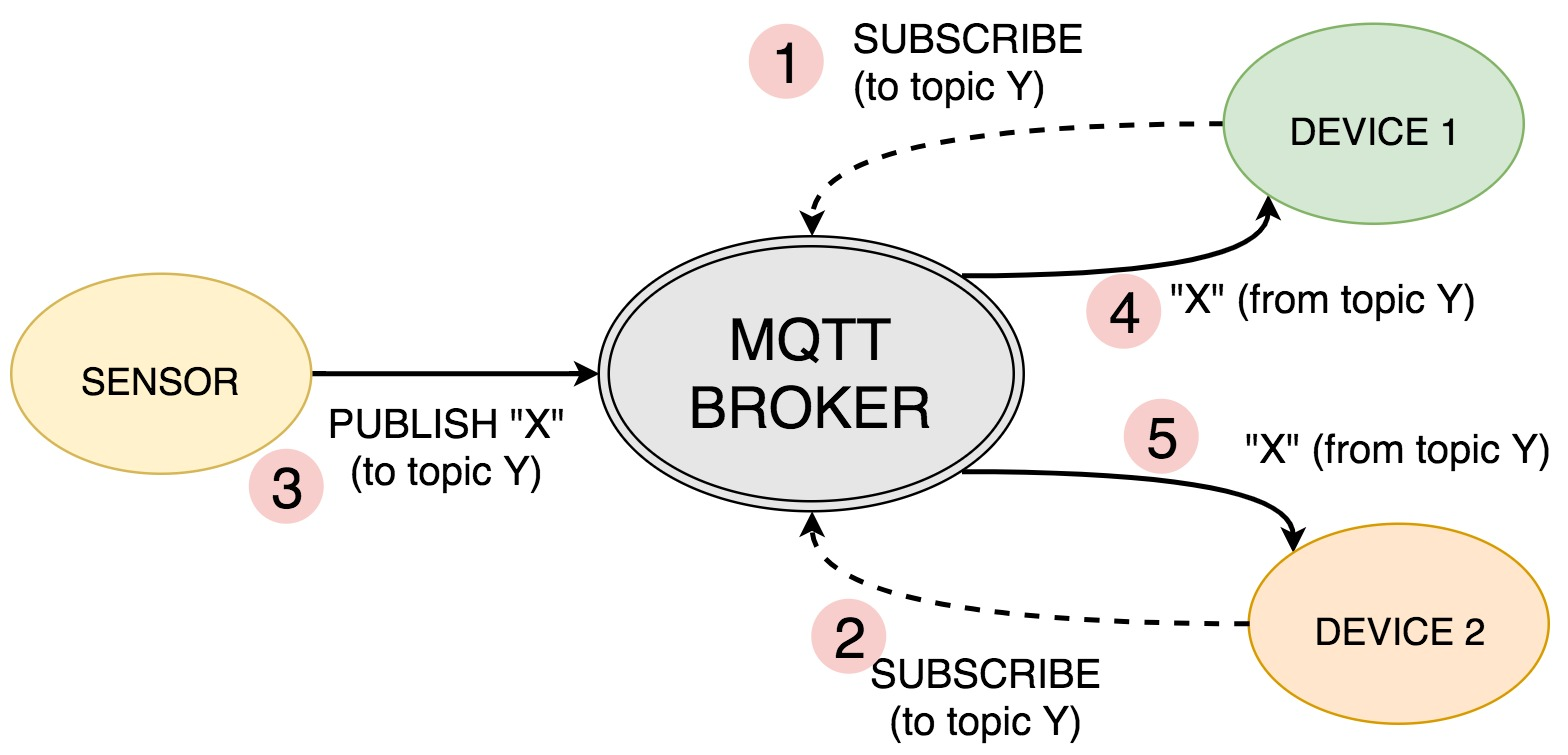
\includegraphics[width=0.7\textwidth]{img/mqtt-communication.jpeg}
    \caption{Ukázka komunikace MQTT \cite{img-mqtt-communication}}
\end{figure}
\label{mqtt-description}
MQTT se vyvýjí již od roku 1999 a momentálně nejpoužívanější verzí je 3.1.1 pro kterou vznikla specifikace v roce 2014. Protokol primárně běží nad TCP/IP, ale lze využít v jakékoliv síti kde je zaručeno správné pořadí dat, beztrátovost a obousměrnost komunikace. Protokol definuje 2 typy entit: \uv{message broker} a klient. MQTT broker je server, který přijímá všechny zprávy od připojených klientů a přeposílá je příjemncům (klientům). MQTT klient je jakékoliv zařízení (od embeded až po server), které komunikuje s brokerem přes síť. \cite{mqtt}

Posílaná data jsou hierarchicky rozdělena do tzv. topiců (česky témat). Topic je textový řetězec o maximální délce 65536 Bytů s oddělovačem "/" - ukázka "/house/bedroom/light". Pokud klient chce odeslat (publish) data, tak pošle zprávu brokeru s daty a topicem do kterého zpráva patří. Broker potom zprávu odešle všem klientům, kteří jsou přihlášení k odběru (subscribe) z daného tématu. O odběr se klient musí přihlásit a to buď přímo specifikuje plný název topicu nebo částečný s použitím zástupných znaků. MQTT počítá s případnou nespolehlivostí ať koncových zařízení nebo sítě a proto umožňuje klientovy při přihlášení definovat \uv{Last Will and Testament} (\hypertarget{LWT}{LWT}). Při přihlášení klient oznámí téma a zprávu, která se odešla v případě nesprávně odpojeného klienta (výpadek sítě / chyba zařízení). Takto lze notifikovat, že došlo je ztráně spojení s daným klientem. \cite{mqtt}

Broker podporuje 3 třídy QoS (Quality of service), kterou lze specifikovat pro každou zprávu jednotlivě v závisloti na její důležitosti. Seřazeny jsou vzestupně dle náročnosti na systém (overhead) \cite{mqtt}:
\begin{itemize}
    \item \textbf{0 - Maximálně jednou} - zpráva je odeslána pouze jednou a klient ani broker nijak nepotvrzují její přjetí
    \item \textbf{1 - Alespoň jednou} - zpráva je odeslaná několikanásobně, dokud není potvrzené její přijetí
    \item \textbf{2 - Právě jednou} - odesílatel a příjemnce navazují dvoucestný hand-shake, aby bylo zaručeno přijmutí zprávy právě jednou
\end{itemize}


\subsubsection{Výhody jednotného jazyku}
Využití jednotného jazyka pro vývoj Backendu a Frontendu přináší obrovskou výhodu v podobě možnosti sdílet nejenom definice pro objekty, ale i přímo části kódu. Toto je velmi vhodné například pro jednotné validace formulářů, různé datové transformace a sdílení aplikační logiky pro frontend \uv{optimistické aktualizace} (aktuální trend, nečekat na potvrzení požadavku ze serveru, ale rozhraní aktualizivat, jako by požadavek byl úspěšný a pouze v případě neúspěchu zobrazit stav ze serveru). Dále jednotný jazyk umožňuje programátorům při vývoji v případě potřeby pohodlně pracovat na obou částech aplikace aniž by se museli učit nový jazyk.


\subsubsection{Backend}    %https://nodejs.org/en/docs/
%spousta jazyků, pro koncepsi asynchroních messages MQTT a Websocket se hodí NodeJS
Vzhledem k povaze MQTT, který je koncepčně založený na asynchroních zprávách jsem si zvolil technologii NodeJS, která je postavené na asynchroní event-driven architektuře \cite{nodejs}. NodeJS je prostředí pro běh JavaScriptu na straně serveru, kterému se v posledních letech dostává velké pozornosti kvůli jeho oblíbenosti mezi vývojáři, je extrémně přívětivý k začínajícím programátorům a má pozvolnou křivkou učení. Díky své architektuře nabízí velice elegantní přístup pro zpracování akcí, kde se musí čekat na výsledek jako např. u síťové komunikace. V tradičním jazyce jako Java nebo C++ se toto čekaní musí řešit pracným vyvtvořením nového vlákna, které čeká na výsledek a následným zpracováním. V NodeJS je programátor od této problematiky odstíněn a může se tak plně věnovat tvorbě aplikační logiky aniž by měl znalosti a zkušenosti s více vláknovým programováním - kvůli této výhodě preferuji NodeJS kdykoliv kdy je potřeba řešit síťovou či asynchronní komunikaci.

%https://vegibit.com/what-is-nodejs/ 
\paragraph{NodeJS} má pravděpodobně aktuálně největší a nejaktivější komunitu ze všech jazyků. Pro správu knihoven používá balíčkovací systém npm (jsou i jiné alternativy) ze kterého se stal největší ekosystém na světě, který je zastřešený neziskovou společností \uv{npm, Inc.} provozující centrální repozitář se všemi dostupnými moduly pro NodeJS. Díky sve centralizaci je velmi jednoduchý na používání, ale v posledních letech kdy se NodeJS zpopularizoval a nyní se JavaScript stal jedním z nejoblíbenější jazyky \cite{survey-languages}, se ukázala centralizace jako poměrně nešťastné řešení, kvůli vysokým nákladům na provoz infrastruktury. Pro představu velikosti ekosystému: npm v roce 2020 obsahoval 1 200 000 modulů a druhý největší systém RubyGems \uv{pouhých} 350 000 \cite{modulecounts}. Všechny moduly jsou k dispozici zcela zdarma a díky takto aktivní komunitě lidí, kteří dávají k dispozici své knihovny ostatním, je vysoce pravděpodobné, že pokud chceme řešit nějaký problém, tak na něj již existuje knihovna.

\paragraph{TypeScript} je superset JavaScriptu, který navíc přidává komplexní typový systém \cite{ts} a rozhodl jsem se ho využít jako hlavní programovací jazyk pro frontend i backend. Jedná se o OpenSource jazyk vyvýjený společností Microsoft, který jeho vznikem chtěl usnadnit přechod C\# a .NET vývojářum k webovým aplikacím \cite{ts}. Mnoho lidí z JavaScript komunity považuje TypeScript jako kontroverzní počin, protože přidává složitost k velmi elegantnímu jazyku a zvyšuje časovou náročnost vývoje. Já jsem dlouho dobu tento názor také zastával, ale v posledních letech při práci na větších projektech a díky zkušeností z jiných jazyků (včetně striktně typových jako C++ a Java), jsem změnil svůj názor ve prospěch TypeScriptu. Souhlasím, že na první pohled prodlužuje dobu vývoje. Programátor musí psát věci navíc oproti čistému JavaScriptu, ale v dlouhodobém životním cyklu se tato práce \uv{na víc} mnohonásobně vrátí. A to v podobě statické kontroly typů, která minimalizuje riziko pádu aplikace a umožňuje  lepší statickou analýzu kódu, a dále jako největší přínost pro mne jako programátora TypeScript přináší funkční \uv{našeptávání} ve vývojovém prostředí, které pro JavaScriptu i přes veškeré snahy bohužel funguje ve velmi omezené míře.

%https://expressjs.com/
\paragraph{ExpressJS} je velmi minimalistický webový framework (první verze v roce 2010), který je do dnes velmi oblíbený a v mnohém ovlivnil vývoj většiny frameworků. Jeho největší výhoda je vysoká flexibilita. Nabízí pouze základní definici způsobu pracování s HTTP požadavky a možnost registrovat tzv. middleware - software, který rozšiřuje funkcionalitu. Veškerá funkcionalita je dodávána pomocí middlewarů, které jsou k dispozici jako moduly. Vývojář si tedy může výsledný server poskládat přesně dle svých představ, kterých existují desítky vytvořených přímo od autorů a další stovky od komunity. \cite{expressjs}


\paragraph{AgendaJS} je knihovna na perzistentní plánování úkolů (jobs) pro NodeJS \cite{agendajs}. Podporuje zpracování/plánování/perzistenci úkolů a jejich opětovné zpracování v případě chyby  \cite{agendajs}. Tato knihovna bude primárně využita pro zajištění odeslání emailů a pro spouštění případných plánovaných akcí. Proč v souvislosti s odesláním emailů? Jejich zpracování je závislé na třetí straně - emailovém serveru, který nemusí být vždy dostupný. Pokud systém bude mět odeslat email, tak tímto způsobem bude zajištěno, že i v případě selhání bude email opětovně odeslán jakmile bude možné.

\paragraph{Socket.IO} knihovna umožnující navázíní obousměrného spojení s kompatibilním klientem. Je založený na vlastním protokolu využívající HTTP spojení nebo WebSocket a vyznačuje se vysokou spolehlivostí a rychlostí umožňující real-time komunikaci. Jedná se o velice populární a časem ověřené řešení, které zajišťuje kompatibilitu i s prohlížeči nepodporující moderní technologii WebSocket.


\subsubsection{Frontend}
% React + Redux
Prvním světoznámím průkopníkem ve světě JavaScriptu pro tvorbu uživatelského rozhraní byla knihovna jQuery, která existuje do dnes, ale spíše se již považuje za přežitek doby. Dnes existuje obrovské množství Frameworků a knihoven pro tvorbu frontendu, ať pro tvorbu na straně serveru nebo přímo na straně uživatele v JavaScriptu. Trend dnešní doby je přesouvat generování rozhraní na stranu uživatele, jak kvůli snížení výkonostních nároků na server, tak spíše kvůli lepší odezvě a uživatelskému zážitků. Mezi nejznámější JavaScriptové frameworky patří bezpochyby Angular, Vue.js, Svelte a nesmím zapomenout na React, který je sice knihovna, ale řadí se na stejnou úroveň. Já jsem si zvolil jako hlavní prostředek pro tvorbu rozhraní React, právě proto že se jedná o knihovnu. Framework se vyznačuje tím, že vynucuje určité problémy řešit jistým způsobem bez možnosti volby. Má to své výhody a nevýhody a do větších týmu bych rozhodně volil raději Framework. Tento projekt ale budu vytvářet primárně sám a mám velice rád flexibilitu a možnost volby. V začátcích to bývá časově náročnější, ale vidím v tom obrovskou možnost osobního růstu, protože při každé volbě musím hodnoti výhody/nevýhody a nakonec retrospektivně vidím následky svých rozhodnutí. Mimo to je React vytvářet společností Facebook a používán největšími technologickými spočnostmi světa (Facebook, Nextflix a Airbnb \cite{react-companies}), takže je jistá jeho dlouhodobá podpora a od roku 2013, kdy byla vydána první verze je dobře odladěný a ověřený.

%https://reactjs.org/tutorial/tutorial.html#what-is-react
\paragraph{React} je deklarativní, efektivní a flexibilní JavaScriptová knihovna pro tvorbu uživatelského rozhraní. Kód dělí do malých izolovaných částí nazvaných \uv{komponenty}, které se skládání do sebe a mohou tvořit komplexní uživatelská rozhraní. Pro vysoký výkon využívá techniku virtuálního DOM - nejprve si vytvoří virtuální strom podoby rozhraní v paměti, který následně porovná s aktuální podobou vykreslenou v prohlížeči a zmanipuluje pouze ty části které se od posledního vykreslení změnily. Díky tomu je velice efektivní a dokáže vykreslovat komplexní stránky s obrovským množstvím dat. \cite{react}


%\section{Návrh uživatelského rozhraní}